\subsection{Энергия системы зарядов. Поле объемного заряда. Энергия и плотность энергии ЭС поля}

\begin{definition}
    Энергия системы зарядов.

    Для образования любой системы заряженных тел необходимо совершить работу, т.к. заряды взаимодействуют между собой по закону Кулона. 
    Установим работу по перемещению заряда из бесконечности в заданную точку пространства. 

    Работа по переносу заряда $q_1$ из бесконечности в точку 1 будет равняться нулю, т.к. на данный момент электрическое поле в выбранной 
    точке пространства отсутствует:

    $$A_1 = 0$$
\end{definition}

Работа по перемещению заряда $q_2$ равна произведению его величины на разность потенциалов в точке 1 и точке 2. 
Потенциал в точке 1 (= $\infty$) равен нулю, тогда:

$$A_2=q_2(\varphi_2-\varphi_\infty)=q_2\varphi_2=k\frac{q_1q_2}{r_{12}}$$

Для переноса заряда $q_3$ в точку 3 необходимо выполнить работу против сил поля, созданного уже двумя зарядами $q_1\ и\ q_2$:

$$A_3=q_3(\phi_3 - \phi_\infty) = q_3\phi_3 = q_3 \left( k\frac{q_1}{r_{13}} + k\frac{q_2}{r_{23}} \right) = k\left( \frac{q_1 q_3}{r_{13}} + \frac{q_2 q_3}{r_{23}} \right)$$

тогда

**Энергия системы** — сумма этих работ:

$$
W=A_1+A_2+\cdots+A_n
$$

для системы из $n$ точечных зарядов:

$$
W=\frac{1}{2}\sum_iq_i\varphi_i
$$

Поле объемных зарядов.

\begin{figure}[h]
    \centering
    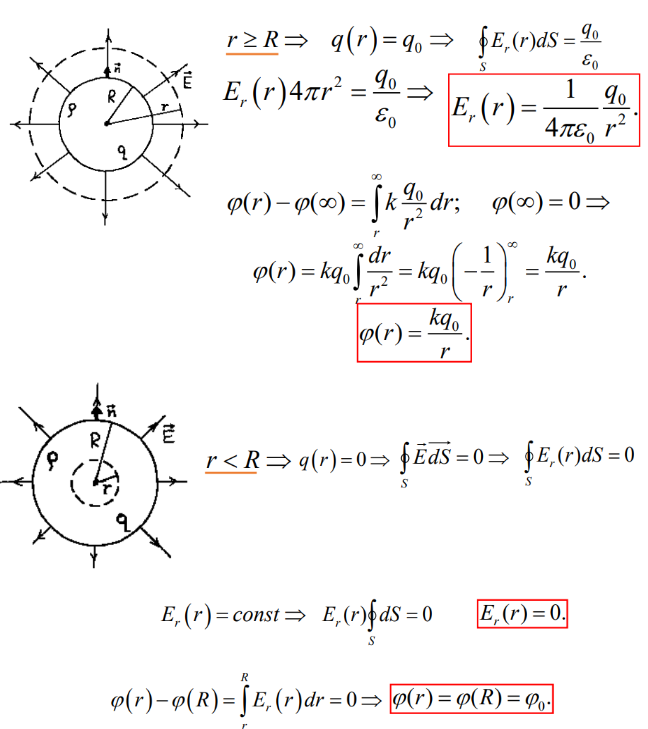
\includegraphics[width=0.5\linewidth]{imgs/q21i1.png}
\end{figure}

Энергия ЭС поля.

Энергия поля конденсатора:

$$
W=\frac{1}{2}\varepsilon\varepsilon_0SdE^2,
$$

где $Sd=V$ — объем пространства, в котором сосредоточено поле

Плотность энергии ЭС поля — физическая величина, численно равная энергии ЭС поля, сосредоточенного в единице объема пространства:

$$
\omega=\frac{W}{V}=\frac{1}{2}\varepsilon\varepsilon_0E^2=\frac{D^2}{2\varepsilon\varepsilon_0}=\frac{ED}{2},
$$

где $D=\varepsilon\varepsilon_0E$ — вектор напряженности электрического поля
